\documentclass[]{book}
\usepackage{lmodern}
\usepackage{amssymb,amsmath}
\usepackage{ifxetex,ifluatex}
\usepackage{fixltx2e} % provides \textsubscript
\ifnum 0\ifxetex 1\fi\ifluatex 1\fi=0 % if pdftex
  \usepackage[T1]{fontenc}
  \usepackage[utf8]{inputenc}
\else % if luatex or xelatex
  \ifxetex
    \usepackage{mathspec}
  \else
    \usepackage{fontspec}
  \fi
  \defaultfontfeatures{Ligatures=TeX,Scale=MatchLowercase}
\fi
% use upquote if available, for straight quotes in verbatim environments
\IfFileExists{upquote.sty}{\usepackage{upquote}}{}
% use microtype if available
\IfFileExists{microtype.sty}{%
\usepackage{microtype}
\UseMicrotypeSet[protrusion]{basicmath} % disable protrusion for tt fonts
}{}
\usepackage[margin=1in]{geometry}
\usepackage{hyperref}
\hypersetup{unicode=true,
            pdftitle={Test multivariados de independencia basados en grafos},
            pdfauthor={Hernán David Torres, Olga Lisethe Castellanos  Universidad Nacional de Colombia},
            pdfborder={0 0 0},
            breaklinks=true}
\urlstyle{same}  % don't use monospace font for urls
\usepackage{natbib}
\bibliographystyle{apalike}
\usepackage{color}
\usepackage{fancyvrb}
\newcommand{\VerbBar}{|}
\newcommand{\VERB}{\Verb[commandchars=\\\{\}]}
\DefineVerbatimEnvironment{Highlighting}{Verbatim}{commandchars=\\\{\}}
% Add ',fontsize=\small' for more characters per line
\usepackage{framed}
\definecolor{shadecolor}{RGB}{248,248,248}
\newenvironment{Shaded}{\begin{snugshade}}{\end{snugshade}}
\newcommand{\KeywordTok}[1]{\textcolor[rgb]{0.13,0.29,0.53}{\textbf{#1}}}
\newcommand{\DataTypeTok}[1]{\textcolor[rgb]{0.13,0.29,0.53}{#1}}
\newcommand{\DecValTok}[1]{\textcolor[rgb]{0.00,0.00,0.81}{#1}}
\newcommand{\BaseNTok}[1]{\textcolor[rgb]{0.00,0.00,0.81}{#1}}
\newcommand{\FloatTok}[1]{\textcolor[rgb]{0.00,0.00,0.81}{#1}}
\newcommand{\ConstantTok}[1]{\textcolor[rgb]{0.00,0.00,0.00}{#1}}
\newcommand{\CharTok}[1]{\textcolor[rgb]{0.31,0.60,0.02}{#1}}
\newcommand{\SpecialCharTok}[1]{\textcolor[rgb]{0.00,0.00,0.00}{#1}}
\newcommand{\StringTok}[1]{\textcolor[rgb]{0.31,0.60,0.02}{#1}}
\newcommand{\VerbatimStringTok}[1]{\textcolor[rgb]{0.31,0.60,0.02}{#1}}
\newcommand{\SpecialStringTok}[1]{\textcolor[rgb]{0.31,0.60,0.02}{#1}}
\newcommand{\ImportTok}[1]{#1}
\newcommand{\CommentTok}[1]{\textcolor[rgb]{0.56,0.35,0.01}{\textit{#1}}}
\newcommand{\DocumentationTok}[1]{\textcolor[rgb]{0.56,0.35,0.01}{\textbf{\textit{#1}}}}
\newcommand{\AnnotationTok}[1]{\textcolor[rgb]{0.56,0.35,0.01}{\textbf{\textit{#1}}}}
\newcommand{\CommentVarTok}[1]{\textcolor[rgb]{0.56,0.35,0.01}{\textbf{\textit{#1}}}}
\newcommand{\OtherTok}[1]{\textcolor[rgb]{0.56,0.35,0.01}{#1}}
\newcommand{\FunctionTok}[1]{\textcolor[rgb]{0.00,0.00,0.00}{#1}}
\newcommand{\VariableTok}[1]{\textcolor[rgb]{0.00,0.00,0.00}{#1}}
\newcommand{\ControlFlowTok}[1]{\textcolor[rgb]{0.13,0.29,0.53}{\textbf{#1}}}
\newcommand{\OperatorTok}[1]{\textcolor[rgb]{0.81,0.36,0.00}{\textbf{#1}}}
\newcommand{\BuiltInTok}[1]{#1}
\newcommand{\ExtensionTok}[1]{#1}
\newcommand{\PreprocessorTok}[1]{\textcolor[rgb]{0.56,0.35,0.01}{\textit{#1}}}
\newcommand{\AttributeTok}[1]{\textcolor[rgb]{0.77,0.63,0.00}{#1}}
\newcommand{\RegionMarkerTok}[1]{#1}
\newcommand{\InformationTok}[1]{\textcolor[rgb]{0.56,0.35,0.01}{\textbf{\textit{#1}}}}
\newcommand{\WarningTok}[1]{\textcolor[rgb]{0.56,0.35,0.01}{\textbf{\textit{#1}}}}
\newcommand{\AlertTok}[1]{\textcolor[rgb]{0.94,0.16,0.16}{#1}}
\newcommand{\ErrorTok}[1]{\textcolor[rgb]{0.64,0.00,0.00}{\textbf{#1}}}
\newcommand{\NormalTok}[1]{#1}
\usepackage{longtable,booktabs}
\usepackage{graphicx,grffile}
\makeatletter
\def\maxwidth{\ifdim\Gin@nat@width>\linewidth\linewidth\else\Gin@nat@width\fi}
\def\maxheight{\ifdim\Gin@nat@height>\textheight\textheight\else\Gin@nat@height\fi}
\makeatother
% Scale images if necessary, so that they will not overflow the page
% margins by default, and it is still possible to overwrite the defaults
% using explicit options in \includegraphics[width, height, ...]{}
\setkeys{Gin}{width=\maxwidth,height=\maxheight,keepaspectratio}
\IfFileExists{parskip.sty}{%
\usepackage{parskip}
}{% else
\setlength{\parindent}{0pt}
\setlength{\parskip}{6pt plus 2pt minus 1pt}
}
\setlength{\emergencystretch}{3em}  % prevent overfull lines
\providecommand{\tightlist}{%
  \setlength{\itemsep}{0pt}\setlength{\parskip}{0pt}}
\setcounter{secnumdepth}{5}
% Redefines (sub)paragraphs to behave more like sections
\ifx\paragraph\undefined\else
\let\oldparagraph\paragraph
\renewcommand{\paragraph}[1]{\oldparagraph{#1}\mbox{}}
\fi
\ifx\subparagraph\undefined\else
\let\oldsubparagraph\subparagraph
\renewcommand{\subparagraph}[1]{\oldsubparagraph{#1}\mbox{}}
\fi

%%% Use protect on footnotes to avoid problems with footnotes in titles
\let\rmarkdownfootnote\footnote%
\def\footnote{\protect\rmarkdownfootnote}

%%% Change title format to be more compact
\usepackage{titling}

% Create subtitle command for use in maketitle
\newcommand{\subtitle}[1]{
  \posttitle{
    \begin{center}\large#1\end{center}
    }
}

\setlength{\droptitle}{-2em}
  \title{Test multivariados de independencia basados en grafos}
  \pretitle{\vspace{\droptitle}\centering\huge}
  \posttitle{\par}
  \author{Hernán David Torres, Olga Lisethe Castellanos Universidad Nacional de
Colombia}
  \preauthor{\centering\large\emph}
  \postauthor{\par}
  \predate{\centering\large\emph}
  \postdate{\par}
  \date{lunes, 27 de noviembre de 2017}

\usepackage{booktabs}
\usepackage{amsthm}
\usepackage{amssymb}
\usepackage{amsmath}
\usepackage{mathspec}
\providecommand{\abs}[1]{\lvert#1\rvert}
\makeatletter
\def\thm@space@setup{%
  \thm@preskip=8pt plus 2pt minus 4pt
  \thm@postskip=\thm@preskip
}
\makeatother

\begin{document}
\maketitle

{
\setcounter{tocdepth}{1}
\tableofcontents
}
\chapter{INTRODUCCIÓN}\label{introduccion}

\begin{quote}
Se exponen, a continuación, algunos test multivariados de independencia,
basados en grafos, entre dos vectores aleatorios de dimensión arbitraria
usados, convenientemente, en situaciones de \emph{\emph{HDLSSD}}.
\citep{sarkar2017some}
\end{quote}

\chapter{¿QUÉ ES HDLSSD?}\label{intro}

Previo a lo anterior, es importante mencionar que \emph{\emph{High
Dimensional Low Sample Size Data}} \emph{\emph{HDLSSD}} refiere, como su
nombre lo indica, a las situaciones en las cuales se tiene alta
dimensionalidad (gran cantidad de variables) y tamaños muestrales
pequeños.

\chapter{EL PROBLEMA}\label{el-problema}

Se han desarrollado muchos test estadísticos ---tanto paramétricos como
no paramétricos --- para probar la independencia entre 2 vectores
aleatorios, pero dichos test no son aplicables en casos de alta
dimensionalidad y de muestras pequeñas.

\section{Desarrollo teórico}\label{desarrollo-teorico}

En las situaciones tratadas se consideran \emph{\emph{n}} realizaciones
independientes,

\[
 z_{1} =
\begin{pmatrix} x_1\\
y_1\\
\end{pmatrix} 
 ,  z_{2} =
\begin{pmatrix} x_2\\
y_2\\
\end{pmatrix}, ... ,    z_{n} =
\begin{pmatrix} x_n\\
y_n\\
\end{pmatrix},
\]

de un vector aleatorio continuo \[ Z = \mathbf{\begin{pmatrix} X\\
Y\\
\end{pmatrix}},\] donde \(\mathbf{X}\) \(\in\) \(\mathcal{X}\)
\(\subseteq\) \(\mathbb{R}^p\) y \(Y\) \(\in\) \(\mathcal{Y}\)
\(\subseteq\) \(\mathbb{R}^q\)

\section{Test existentes}\label{test-existentes}

\begin{longtable}[]{@{}ccl@{}}
\caption{Parangón de los test propuestos hasta el
momento.}\tabularnewline
\toprule
\begin{minipage}[b]{0.25\columnwidth}\centering\strut
\emph{Test paramétricos}\strut
\end{minipage} & \begin{minipage}[b]{0.10\columnwidth}\centering\strut
\strut
\end{minipage} & \begin{minipage}[b]{0.56\columnwidth}\raggedright\strut
\emph{Test no paramétricos}\strut
\end{minipage}\tabularnewline
\midrule
\endfirsthead
\toprule
\begin{minipage}[b]{0.25\columnwidth}\centering\strut
\emph{Test paramétricos}\strut
\end{minipage} & \begin{minipage}[b]{0.10\columnwidth}\centering\strut
\strut
\end{minipage} & \begin{minipage}[b]{0.56\columnwidth}\raggedright\strut
\emph{Test no paramétricos}\strut
\end{minipage}\tabularnewline
\midrule
\endhead
\begin{minipage}[t]{0.25\columnwidth}\centering\strut
Basado en el estadístico Wilk\strut
\end{minipage} & \begin{minipage}[t]{0.10\columnwidth}\centering\strut
\emph{\emph{Univariados}}\strut
\end{minipage} & \begin{minipage}[t]{0.56\columnwidth}\raggedright\strut
Estadístico de Spearman \(\rho\) y Estadístico de Kendall \(\tau\)\strut
\end{minipage}\tabularnewline
\begin{minipage}[t]{0.25\columnwidth}\centering\strut
Prueba de la raíz más grande de Roy\strut
\end{minipage} & \begin{minipage}[t]{0.10\columnwidth}\centering\strut
\strut
\end{minipage} & \begin{minipage}[t]{0.56\columnwidth}\raggedright\strut
Test basado en cuadrantes estadísticos\strut
\end{minipage}\tabularnewline
\begin{minipage}[t]{0.25\columnwidth}\centering\strut
Traza de Hotelling-Lawley\strut
\end{minipage} & \begin{minipage}[t]{0.10\columnwidth}\centering\strut
\emph{\emph{Multivariados}}\strut
\end{minipage} & \begin{minipage}[t]{0.56\columnwidth}\raggedright\strut
Extensión del test de cuadrantes para mayores dimensiones mediantes
interdirecciones\strut
\end{minipage}\tabularnewline
\begin{minipage}[t]{0.25\columnwidth}\centering\strut
Traza de Pillai-Bartlett\strut
\end{minipage} & \begin{minipage}[t]{0.10\columnwidth}\centering\strut
\strut
\end{minipage} & \begin{minipage}[t]{0.56\columnwidth}\raggedright\strut
Generalizaciones multivariadas de los test basados en Spearman y
Kendall.\strut
\end{minipage}\tabularnewline
\begin{minipage}[t]{0.25\columnwidth}\centering\strut
\strut
\end{minipage} & \begin{minipage}[t]{0.10\columnwidth}\centering\strut
\strut
\end{minipage} & \begin{minipage}[t]{0.56\columnwidth}\raggedright\strut
Generalizaciones del cuadrante estadístico usando signos espaciales y
rangos\strut
\end{minipage}\tabularnewline
\bottomrule
\end{longtable}

\section{Test aplicables a HDLSS}\label{test-aplicables-a-hdlss}

Para manipular datos HDLSS en distintas áreas de investigación, se han
desarrollado algunos test de independencia entre dos vectores, basados
en grafos y enfocados en distancias \emph{inter-point}; sea \(d_{x}\) y
\(d_{y}\) medidas de distancia en \(\mathcal{X}\) y \(\mathcal{Y}\),
respectivamente; y, para toda \((i,j)\), definimos
\[ d_{ij}^x = d_x(x_i, x_j), \\ d_{ij}^y = d_y(y_i, y_j). \]

En la mayoría de los test presentados, a continuación, se utiliza
distancias euclidianas en \(\mathcal{X}\) y \(\mathcal{Y}\) como
\(d_{x}\) y \(d_{y}\) , respectivamente.

\chapter{Teoría de grafos}\label{teoria-de-grafos}

\section{Generalidades}\label{generalidades}

\begin{itemize}
\tightlist
\item
  Rama de las matemáticas y las ciencias de la computación que estudia
  las propiedades de los grafos
\item
  Un grafo \(\displaystyle G=(V,E)\) es una pareja ordenada en la que
  \(\mathbf{V}\) es un conjunto no vacío de \textbf{vértices} y
  \(\mathbf{E}\) es un conjunto de \textbf{aristas}.

  \begin{itemize}
  \tightlist
  \item
    \(\mathbf{V}\) consta de pares no ordenados de vértices, tales como
    \$\{x,y\} \in E \$, entonces decimos que \(x\) e \(y\) son
    adyacentes.
  \end{itemize}
\end{itemize}

\section{Un poco de historia}\label{un-poco-de-historia}

\begin{itemize}
\item
  Siglo XVIII: Problema de los puentes de \emph{Königsberg}: Encontrar
  un camino que recorriera los siete puentes del río Pregel,de modo que
  se recorrieran todos los puentes pasando una sola vez por cada uno de
  ellos.
\item
  1736: El trabajo de Leonhard Euler sobre el problema titulado ``La
  solución de un problema relativo a la geometría de la posición'' es
  considerado el primer resultado de la teoría de
  grafos.\citep{euler1741solutio}
\end{itemize}

\begin{figure}

{\centering 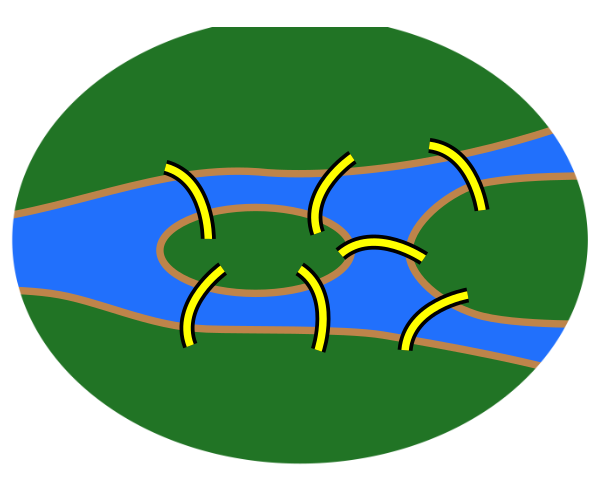
\includegraphics[width=360,height=500]{7_bridges} 

}

\caption{Los siete puentes del río Pregel}\label{fig:unnamed-chunk-1}
\end{figure}

\section{Composición y conceptos}\label{composicion-y-conceptos}

\begin{itemize}
\item
  \textbf{\emph{Grafo simple o grafo:}} Conjunto de \emph{nodos} unidos
  por enlaces llamados \emph{aristas}.
\item
  \textbf{\emph{Grafo completo}}: Grafo simple donde \emph{cada par de
  vértices} está conectado por una \emph{arista}. Tiene \(n(n-1)/2\)
  aristas. Grafo regular de grado \(n-1\)
\item
  \textbf{\emph{Camino:}} Secuencia de vértices dentro de un grafo tal
  que exista una arista entre cada vértice y el siguiente.
\end{itemize}

\begin{figure}

{\centering 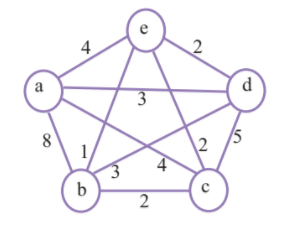
\includegraphics[width=260,height=240]{grafo_completo} 

}

\caption{Grafo completo ponderado}\label{fig:unnamed-chunk-2}
\end{figure}

\section{Tipos de grafos}\label{tipos-de-grafos}

\begin{itemize}
\item
  \textbf{\emph{Subgrafo:}} Cuyo conjunto de vértices(como el de
  aristas) es un subconjunto del de grafo original.
\item
  \textbf{\emph{Grafo de arcos ponderados o etiquetado}}: Grafo con
  asignaciones de pesos en cada arco.
\item
  \textbf{\emph{Árbol:}} Donde cualesquiera dos vértices están
  conectados por exactamente \emph{un camino}.
\end{itemize}

\begin{figure}

{\centering 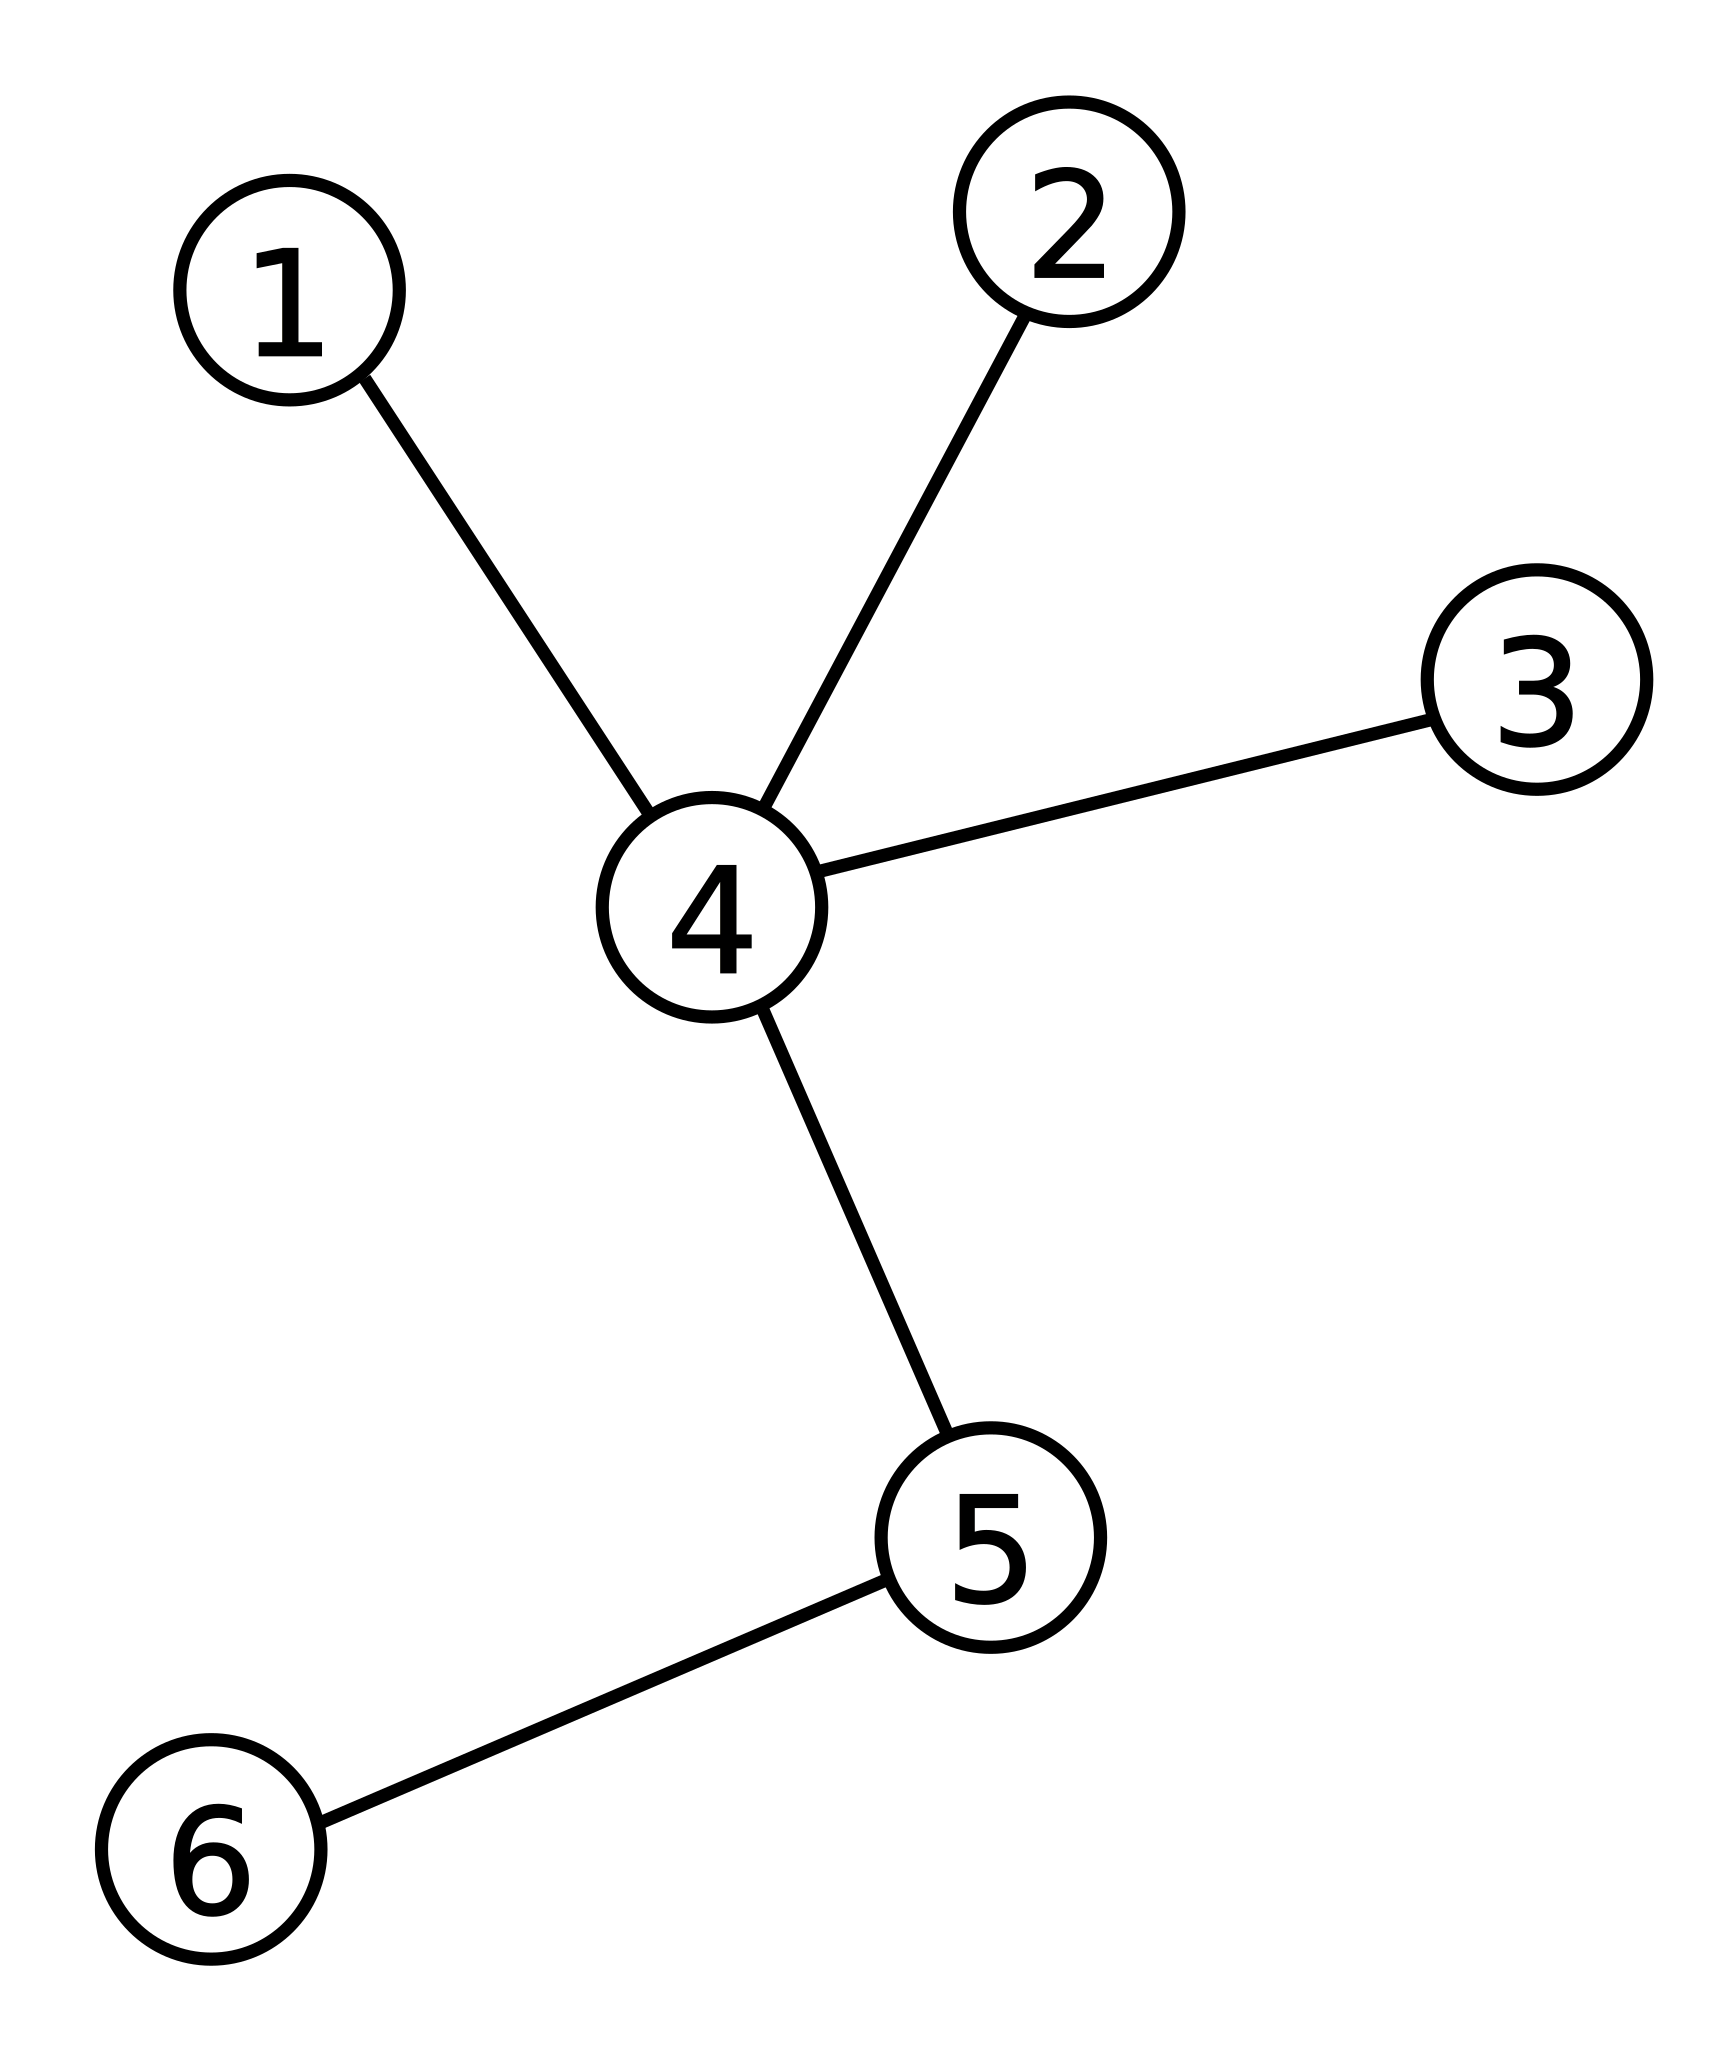
\includegraphics[width=260,height=240]{Tree_graph} 

}

\caption{Árbol}\label{fig:unnamed-chunk-3}
\end{figure}

\section{Ejemplo básico en R}\label{ejemplo-basico-en-r}

\begin{Shaded}
\begin{Highlighting}[]
\KeywordTok{library}\NormalTok{(igraph)}
\NormalTok{g <-}\StringTok{ }\KeywordTok{graph.formula}\NormalTok{(}\DecValTok{1}\OperatorTok{-}\DecValTok{2}\NormalTok{, }\DecValTok{1}\OperatorTok{-}\DecValTok{3}\NormalTok{ ,}\DecValTok{1}\OperatorTok{-}\DecValTok{4}\NormalTok{, }\DecValTok{1}\OperatorTok{-}\DecValTok{5}\NormalTok{ , }\DecValTok{1}\OperatorTok{-}\DecValTok{6}\NormalTok{ ,}\DecValTok{1}\OperatorTok{-}\DecValTok{7}\NormalTok{, }\DecValTok{2}\OperatorTok{-}\DecValTok{6}\NormalTok{, }\DecValTok{2}\OperatorTok{-}\DecValTok{7}\NormalTok{, }\DecValTok{3}\OperatorTok{-}\DecValTok{5}\NormalTok{, }\DecValTok{4}\OperatorTok{-}\DecValTok{5}\NormalTok{ ,}\DecValTok{4}\OperatorTok{-}\DecValTok{6}\NormalTok{, }\DecValTok{4}\OperatorTok{-}\DecValTok{7}\NormalTok{, }\DecValTok{5}\OperatorTok{-}\DecValTok{6}\NormalTok{, }\DecValTok{5}\OperatorTok{-}\DecValTok{7}\NormalTok{, }\DecValTok{6}\OperatorTok{-}\DecValTok{7}\NormalTok{)}
\CommentTok{# V(g) Muestra las etiquetas vértices del grafo}
\CommentTok{# E(g) Muestra los arcos del grafo}
\KeywordTok{plot}\NormalTok{(g)}
\end{Highlighting}
\end{Shaded}

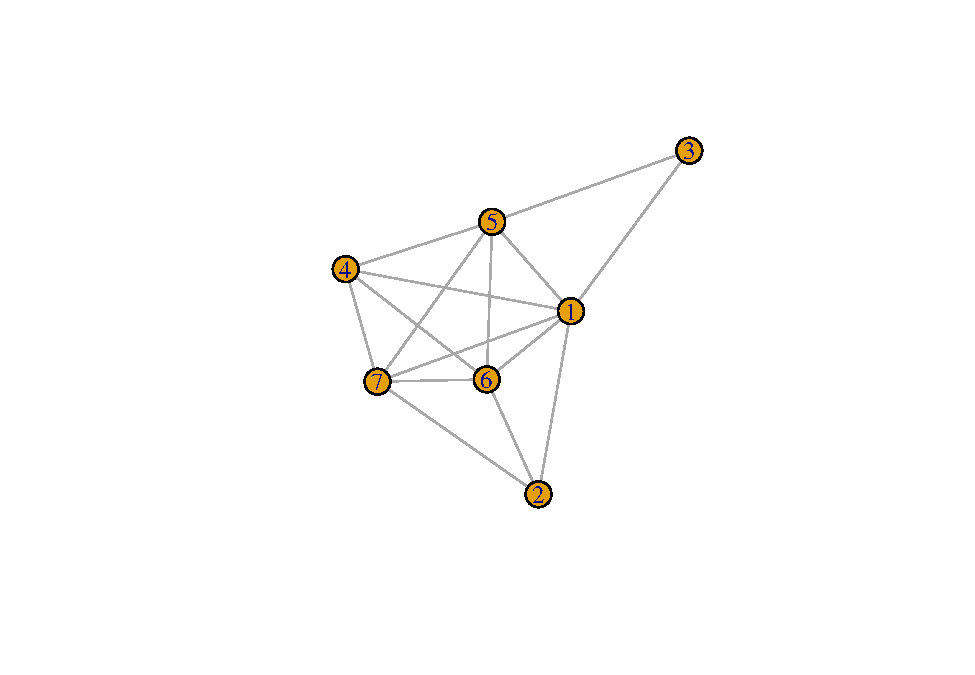
\includegraphics{Tests_files/figure-latex/unnamed-chunk-4-1.pdf}

\chapter{TEST BASADO EN GRAFOS}\label{test-basado-en-grafos}

\section{Precisiones del test}\label{precisiones-del-test}

Se consideran dos grafos completos de arcos ponderados
\(\mathcal{G}_{\mathbf{x}}\) y \(\mathcal{G}_{\mathbf{y}}\) con nodos
\(\mathbf{x_1,...,x_n}\) y \(\mathbf{y_1,..., y_n}\), respectivamente,
donde \(d_{i,j}^{\mathbf{x}}\) (y, correspondientemente,
\(d_{i,j}^{\mathbf{y}}\)) es la ponderación asociada con el lado que
conecta a \(\mathbf{x}_i\) y \(\mathbf{x}_j\) (y, paralelamente, con
\(\mathbf{y}_i\) y \(\mathbf{y}_j\)) \citep{friedman1983graph}

\section{Grafo K vecinos más
próximos}\label{grafo-k-vecinos-mas-proximos}

El gráfico K-NN en \(\mathcal{G}_{\mathbf{x}}\) tiene un arco entre
\(x_i\) y \(x_j\), si \(x_i\) es uno de los primeros K vecinos de
\(x_j\) o viceversa; y, análogamente, para \(\mathcal{G}_{\mathbf{x}}\).

\begin{figure}

{\centering 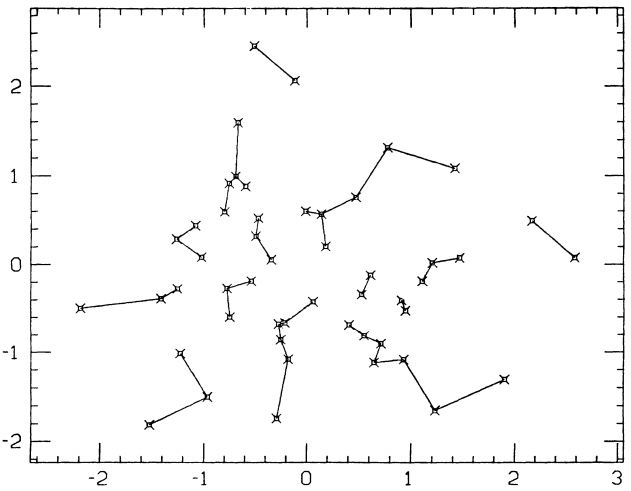
\includegraphics[width=450,height=320]{1-nn} 

}

\caption{1-NN 50 obs. Normal bivariada}\label{fig:unnamed-chunk-5}
\end{figure}

\section{Ejemplo: Grafo 5-NN}\label{ejemplo-grafo-5-nn}

\begin{figure}

{\centering 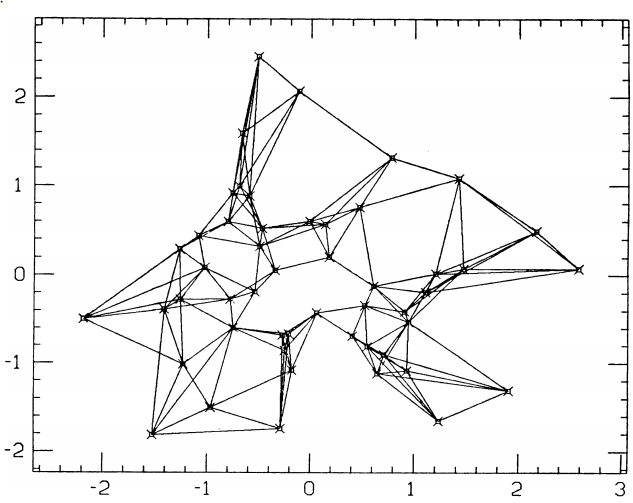
\includegraphics[width=450,height=320]{5-nn} 

}

\caption{5-NN en 50 obs. Normal bivariada}\label{fig:unnamed-chunk-6}
\end{figure}

\section{El árbol recubridor mínimo
(MST)}\label{el-arbol-recubridor-minimo-mst}

Es un subgrafo que tiene que ser un árbol y contener todos los vértices
del grafo inicial y, a la vez, será el de la menor suma de los pesos.

\begin{figure}

{\centering 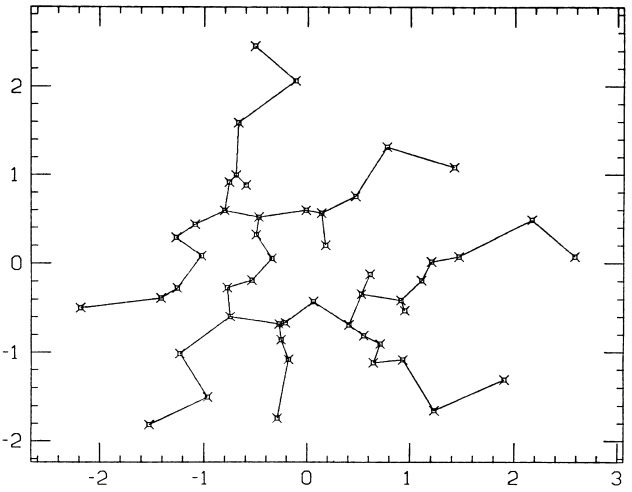
\includegraphics[width=450,height=320]{1-MST} 

}

\caption{1-MST en 50 obs. Normal bivariada}\label{fig:unnamed-chunk-7}
\end{figure}

\section{Ejemplo: Grafo 5-MST}\label{ejemplo-grafo-5-mst}

El r-MST, \(r={1, 2,...,K}\), es un árbol recubridor mínimo que no
comparte arco alguno con ninguno de los r-1 anteriores.

\begin{figure}

{\centering 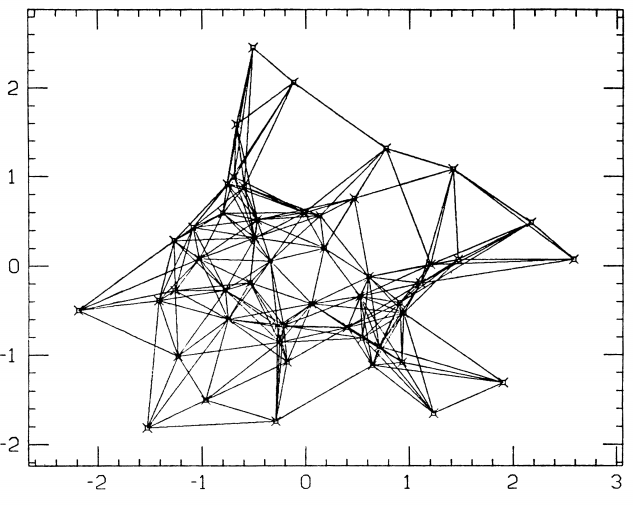
\includegraphics[width=450,height=320]{5-MST} 

}

\caption{5-MST en 50 obs. Normal bivariada}\label{fig:unnamed-chunk-8}
\end{figure}

\section{Test estadístico}\label{test-estadistico}

Sea \(\tau_x^k\) y \(\tau_y^k\) el K-MST o el K-NN sobre el grafo
completo \(\mathcal{G}_{\mathbf{x}}\) y \(\mathcal{G}_{\mathbf{x}}\),
respectivamente.

Se define lo siguiente para determinar el número de arcos en común.

\[a_{ij}=  \left\{
  \begin{array}{ll}
 1 &  \mathcal{Sí} \ (i,j)\in \mathcal{G}_{\mathbf{x}}  \\
 0 &  \mathcal{e.o.c.} \\ 
 \end{array}
\right.
\] De la misma forma se definen los \(b_{i,j}\) basados en las
distancias de \(\mathcal{Y}\).

El estadístico correspondiente es:

\[T_{RF} = \displaystyle \sum_{i=1}^n \sum_{j=1}^n a_{ij}b_{ij}\]

\section{Test estadístico libre de distribución basado en
grafos}\label{test-estadistico-libre-de-distribucion-basado-en-grafos}

\begin{quote}
Pequeñas distancias en \(\mathcal{x}\) corresponden a pequeñas
distancias en \(\mathcal{y}\)
\end{quote}

Seleccionamos un recorrido aleatorio del árbol, donde en cada paso
comenzamos en un nodo ya visitado,\(i \in V= {1,2,...,n}\), y avanzamos
hacia un nuevo nodo,\(j \in V^c\),. Por lo tanto, el árbol se recorre en
\(n-1\) pasos. Se calcula el rango \(R_i\) en cada
\(d_{i,j}^{\mathbf{y}}\) y se obtienen \(n-2\) rangos.

Y se usa el siguiente estadístico

\[T_{RT} =  -2 \displaystyle \sum_{i=1}^{n-2} log(\dfrac{R_j}{n-i})\]

\section{Ejemplo de juguete}\label{ejemplo-de-juguete}

\begin{figure}

{\centering 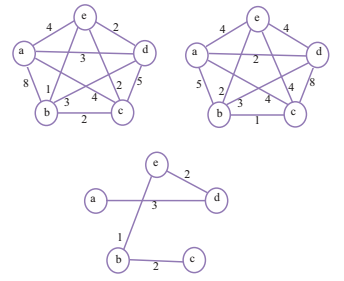
\includegraphics[width=500,height=450]{test6} 

}

\caption{Ejemplo de juguete}\label{fig:unnamed-chunk-9}
\end{figure}

\section{Algoritmo de Prim}\label{algoritmo-de-prim}

Permite encontrar un árbol recubridor mínimo de un grafo no dirigido y
completo. 1. Se selecciona el arco con menor peso. 2. Aumentar el árbol
por un lado: De las posibles uniones que pueden conectar el árbol a los
vértices que no están aún en el árbol, encontrar el lado de menor
distancia y unirlo al árbol. 3. Repetir el paso 2 (hasta que todos los
vértices pertenezcan al árbol) \citep{heller2012consistent}

\section{Ejemplo}\label{ejemplo}

\begin{figure}

{\centering \includegraphics[width=400,height=320]{Minimum_spanning_tree} 

}

\caption{Ejemplo de juguete}\label{fig:unnamed-chunk-10}
\end{figure}

\section{Test modificado libre de
distribución}\label{test-modificado-libre-de-distribucion}

A causa de la selección aleatoria del recorrido, el anterior test puede
determinar inferencias engañosas. Para eso se usa un recorrido
sistemático siguiendo el \emph{algoritmo de Prim}.
\citep{heller2012consistent}

Y se usa el estadístico T\_\{RT\} de la misma notación; en vez de
\(R_i\), se usa \(R_o\) para distiguir la selección sitematizada de la
aleatoria.

\[T^{o} = -2 \displaystyle \sum_{i=1}^{n-2} log \left( \dfrac{R_i^o}{n-i}\right)\]

Sin embargo, los anteriores test se desempeñan deficientemente en caso
de estar \(d_{i,j}^{\mathbf{y}}\) y \(d_{i,j}^{\mathbf{y}}\)
negativamente relacionada. El problema es afrontado haciendo

\[R_i^{r} = n-i+1- R_o^i\] para \(i= 1, 2, ... , n-2\)

Así

\[ T^{r} = -2 \displaystyle \sum_{i=1}^{n-2} log \left( \dfrac{R_i ^r}{n-i}\right)\]

\chapter{EJEMPLO CON DATOS REALES}\label{ejemplo-con-datos-reales}

\begin{figure}
  
  {\centering 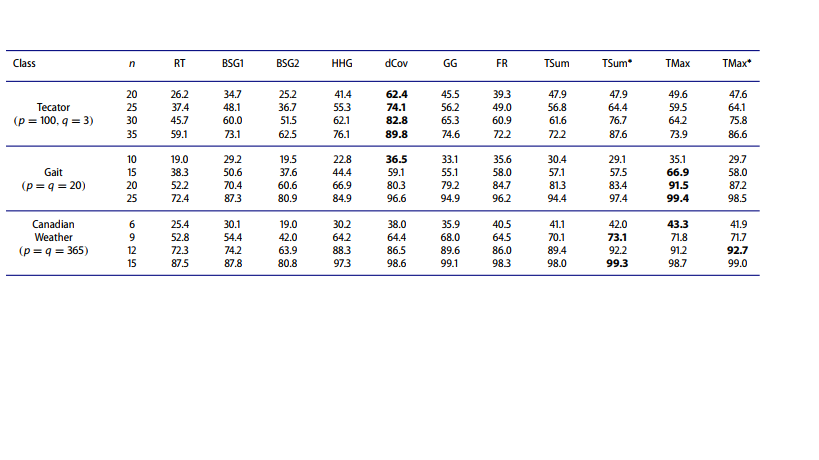
\includegraphics[width=800,height=450]{invento} 
  
  }
  
  \caption{Tabla de contingencia para la clasificación cruzada}\label{fig:unnamed-chunk-11}
  \end{figure}

\chapter{CONCLUSIONES}\label{conclusiones}

\begin{itemize}
\item
  Si bien los test estadísticos presentados al principio se usan para
  probar la independencia, en el caso en el que el número de variables
  supera el de individuos presentan limitaciones o no aplicabilidad; lo
  cual motivó el desarrollo y presentación de métodos basados en grafos,
  los cuales buscan proveer una mejor herramienta para probar
  independencia entre las variables en situaciones de HDLSSD.
\item
  En la construcción del test, se requiere algún tipo de asociación
  entre las x-distancias y las y-distancias, entonces estas relaciones
  se pueden reflejar en sus vecinos más cercanos y el enfoque es llevado
  a buscar proximidades y coincidencias.
\item
  Aunque, para la implementación de los distintos test se utilizó la
  distancia Euclidiana, es posible emplear otro concepto de distancia.
\end{itemize}

\bibliography{book.bib,packages.bib,referencias.bib}


\end{document}
